\documentclass[12pt,a4paper]{report}

% ─────────────────────────── Packages ───────────────────────────
\usepackage[utf8]{inputenc}
\usepackage[T1]{fontenc}
\usepackage{lmodern}
\usepackage[margin=2.5cm]{geometry}
\usepackage{graphicx}
\usepackage{hyperref}
\usepackage{xcolor}
\usepackage{listings}
\usepackage{booktabs}
\usepackage{longtable}
\usepackage{tabularx}
\usepackage{enumitem}
\usepackage{amsmath}
\usepackage{tikz}
\usetikzlibrary{shapes.geometric, arrows.meta, positioning, calc}
\usepackage{fancyhdr}
\usepackage{titlesec}
\usepackage{tocloft}
\usepackage{caption}
\usepackage{float}

% ─────────────────────────── Colors ─────────────────────────────
\definecolor{codebg}{RGB}{245,245,245}
\definecolor{codeframe}{RGB}{200,200,200}
\definecolor{javakey}{RGB}{127,0,85}
\definecolor{javastr}{RGB}{42,0,255}
\definecolor{javacmt}{RGB}{63,127,95}
\definecolor{luakey}{RGB}{0,0,180}
\definecolor{linkblue}{RGB}{0,102,204}

\hypersetup{
    colorlinks=true,
    linkcolor=black,
    urlcolor=linkblue,
    citecolor=black
}

% ─────────────────────────── Listings ───────────────────────────
\lstdefinestyle{JavaStyle}{
    language=Java,
    backgroundcolor=\color{codebg},
    frame=single,
    rulecolor=\color{codeframe},
    basicstyle=\ttfamily\scriptsize,
    keywordstyle=\color{javakey}\bfseries,
    stringstyle=\color{javastr},
    commentstyle=\color{javacmt}\itshape,
    numbers=left,
    numberstyle=\tiny\color{gray},
    numbersep=5pt,
    breaklines=true,
    breakatwhitespace=false,
    tabsize=4,
    showstringspaces=false,
    captionpos=b,
    xleftmargin=1.5em,
    framexleftmargin=1em,
    columns=flexible
}

\lstdefinestyle{LuaStyle}{
    language={[5.3]Lua},
    backgroundcolor=\color{codebg},
    frame=single,
    rulecolor=\color{codeframe},
    basicstyle=\ttfamily\scriptsize,
    keywordstyle=\color{luakey}\bfseries,
    stringstyle=\color{javastr},
    commentstyle=\color{javacmt}\itshape,
    numbers=left,
    numberstyle=\tiny\color{gray},
    numbersep=5pt,
    breaklines=true,
    tabsize=4,
    showstringspaces=false,
    captionpos=b,
    xleftmargin=1.5em,
    framexleftmargin=1em,
    columns=flexible
}

\lstdefinestyle{PropsStyle}{
    backgroundcolor=\color{codebg},
    frame=single,
    rulecolor=\color{codeframe},
    basicstyle=\ttfamily\scriptsize,
    commentstyle=\color{javacmt}\itshape,
    breaklines=true,
    tabsize=4,
    showstringspaces=false,
    captionpos=b,
    xleftmargin=1.5em,
    framexleftmargin=1em,
    columns=flexible
}

\lstset{style=JavaStyle}

% ─────────────────────────── Headers / Footers ──────────────────
\pagestyle{fancy}
\fancyhf{}
\fancyhead[L]{\leftmark}
\fancyhead[R]{Library Management System}
\fancyfoot[C]{\thepage}
\renewcommand{\headrulewidth}{0.4pt}
\renewcommand{\footrulewidth}{0.4pt}

% ─────────────────────────── Title Info ─────────────────────────
\title{
    \vspace{2cm}
    {\Huge\bfseries Library Management System}\\[0.8cm]
    {\Large\itshape Comprehensive Technical Report}\\[1.5cm]
    {\large Distributed Backend Architecture with\\
    Spring Boot, MongoDB, and Redis}\\[2cm]
}
\author{
    \textbf{Project Team}\\[0.3cm]
    Member 1: Core Backend, UI, and Unique ID Generator\\
    Member 2: Redis Cache-Aside, Controlled Crawler, and Search\\
    Member 3: Consistent Hashing and Distributed Storage\\
    Member 4: Token Bucket Rate Limiter and URL Shortener
}
\date{\today}

% ═══════════════════════════════════════════════════════════════
\begin{document}

\maketitle
\thispagestyle{empty}
\newpage

% ─────────────────────────── Abstract ───────────────────────────
\begin{abstract}
This report presents the design, architecture, and implementation of a full-stack \textbf{Library Management System} built with \textbf{Spring Boot 3.3}, \textbf{MongoDB 7.0}, and \textbf{Redis 7.2}. The system demonstrates production-grade distributed systems concepts including a \textbf{Snowflake-based distributed ID generator} with Base62 encoding, a \textbf{Redis-backed Cache-Aside} pattern with hit/miss observability, a \textbf{Consistent Hash Ring} with virtual nodes and MurmurHash3 for storage distribution, a \textbf{Token Bucket Rate Limiter} enforced via atomic Redis Lua scripts, a \textbf{Trie-based autocomplete} engine, a controlled \textbf{web crawler} for catalogue enrichment, and a \textbf{dual-tier URL shortener} with Base62 code generation. The project follows a layered MVC architecture with JWT-based stateless authentication, role-based access control (RBAC), atomic concurrency-safe loan operations, and a responsive web UI. This document covers all technical aspects, data models, algorithms, API endpoints, and key code snippets across the four member contributions.
\end{abstract}

\tableofcontents
\newpage

% ═══════════════════════════════════════════════════════════════
\chapter{Introduction}
% ═══════════════════════════════════════════════════════════════

\section{Project Overview}
The Library Management System is a distributed web application designed to manage books, members, loans, reservations, and fines for a modern library. It is built as a monolithic Spring Boot application with modular service components that demonstrate several advanced data structures and distributed systems concepts.

\section{Objectives}
\begin{itemize}[noitemsep]
    \item Provide CRUD operations for book catalogue management with concurrency-safe borrowing and returning.
    \item Implement a \textbf{Snowflake-based unique ID generator} producing compact, collision-resistant, distributed identifiers.
    \item Build a \textbf{Redis Cache-Aside} layer for sub-millisecond search and book detail caching.
    \item Implement a \textbf{Consistent Hash Ring} with virtual nodes for even key distribution across storage nodes.
    \item Enforce API rate limiting via a \textbf{Token Bucket algorithm} backed by atomic Redis Lua scripts.
    \item Provide \textbf{Trie-based prefix search} for real-time autocomplete suggestions.
    \item Build a controlled \textbf{web crawler} for external catalogue metadata discovery.
    \item Implement a \textbf{dual-tier URL shortener} with Redis + MongoDB persistence.
\end{itemize}

\section{Technology Stack}

\begin{table}[H]
\centering
\caption{Technology Stack Summary}
\begin{tabularx}{\textwidth}{l X}
\toprule
\textbf{Component} & \textbf{Technology} \\
\midrule
Framework & Spring Boot 3.3.4 (Java 17) \\
Database & MongoDB 7.0 (Document Store) \\
Cache / KV Store & Redis 7.2 \\
Authentication & JWT (jjwt 0.12.6) + Spring Security + BCrypt \\
Build Tool & Apache Maven \\
HTML Parsing & Jsoup 1.18.1 \\
Monitoring & Spring Boot Actuator \\
Containerization & Docker Compose \\
Frontend & Vanilla HTML/CSS/JavaScript (served as static resources) \\
\bottomrule
\end{tabularx}
\end{table}

\section{Team Contribution Summary}

\begin{table}[H]
\centering
\caption{Member Contributions}
\begin{tabularx}{\textwidth}{c X}
\toprule
\textbf{Member} & \textbf{Contribution} \\
\midrule
1 & Core backend (Book, Loan, Reservation, Fine CRUD), Web UI, Snowflake ID Generator, JWT Auth \\
2 & Redis Cache-Aside, Controlled Web Crawler, Catalogue Search, Trie Autocomplete \\
3 & Consistent Hash Ring with Virtual Nodes, MurmurHash3, Distribution Analysis, MongoDB Sharding \\
4 & Token Bucket Rate Limiter (Redis Lua), URL Shortener, Base62 Encoding, Rate Limit Admin \\
\bottomrule
\end{tabularx}
\end{table}


% ═══════════════════════════════════════════════════════════════
\chapter{System Architecture}
% ═══════════════════════════════════════════════════════════════

\section{High-Level Architecture}
The system follows a \textbf{layered MVC architecture}:

\begin{center}
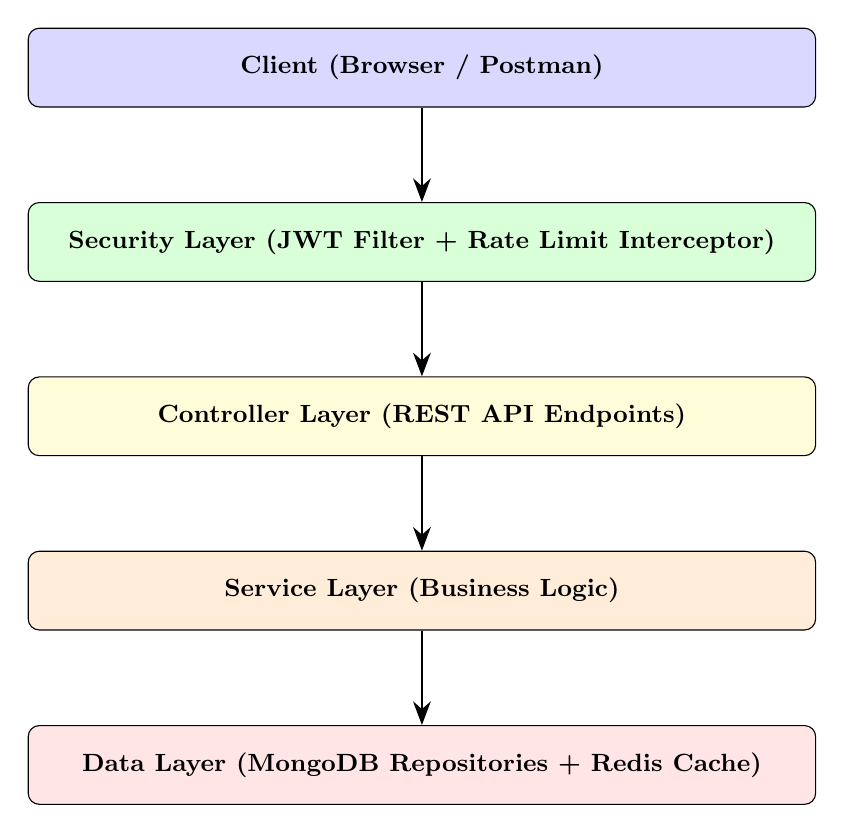
\begin{tikzpicture}[
    box/.style={rectangle, draw, rounded corners, minimum width=10cm, minimum height=1cm, text centered, font=\small\bfseries},
    arrow/.style={-{Stealth[length=3mm]}, thick},
    node distance=1.2cm
]
    \node[box, fill=blue!15] (client) {Client (Browser / Postman)};
    \node[box, fill=green!15, below=of client] (security) {Security Layer (JWT Filter + Rate Limit Interceptor)};
    \node[box, fill=yellow!15, below=of security] (controller) {Controller Layer (REST API Endpoints)};
    \node[box, fill=orange!15, below=of controller] (service) {Service Layer (Business Logic)};
    \node[box, fill=red!10, below=of service] (data) {Data Layer (MongoDB Repositories + Redis Cache)};

    \draw[arrow] (client) -- (security);
    \draw[arrow] (security) -- (controller);
    \draw[arrow] (controller) -- (service);
    \draw[arrow] (service) -- (data);
\end{tikzpicture}
\end{center}

\section{Package Structure}
The source code is organized into the following packages under \texttt{com.library}:

\begin{table}[H]
\centering
\caption{Package Organization}
\begin{tabularx}{\textwidth}{l X}
\toprule
\textbf{Package} & \textbf{Purpose} \\
\midrule
\texttt{config} & Security, Redis, WebMvc, Crawler configuration, Data initializer \\
\texttt{controller} & 13 REST controllers handling all API endpoints \\
\texttt{crawler} & URL validation and HTML catalogue parsing components \\
\texttt{distribution} & ConsistentHashRouter and MurmurHash3 implementation \\
\texttt{dto} & 28 Data Transfer Objects for request/response payloads \\
\texttt{exception} & Custom exceptions and global exception handler \\
\texttt{idgenerator} & Snowflake and TSID ID generation strategies \\
\texttt{model} & 10 MongoDB document entities (Book, Loan, Member, etc.) \\
\texttt{repository} & 6 Spring Data MongoDB repository interfaces \\
\texttt{security} & JWT token provider and authentication filter \\
\texttt{service} & 14 service classes with core business logic \\
\texttt{trie} & Trie (prefix tree) data structure implementation \\
\bottomrule
\end{tabularx}
\end{table}

\section{Source Code Statistics}
\begin{itemize}[noitemsep]
    \item \textbf{Production source files:} 95 Java classes
    \item \textbf{Test source files:} 11 test classes
    \item \textbf{Controllers:} 13
    \item \textbf{Services:} 14
    \item \textbf{DTOs:} 28
    \item \textbf{MongoDB Collections:} 6 (books, members, loans, reservations, fine\_transactions, short\_links)
\end{itemize}


% ═══════════════════════════════════════════════════════════════
\chapter{Data Models}
% ═══════════════════════════════════════════════════════════════

\section{Book Entity}
The \texttt{Book} document represents a library catalogue item stored in MongoDB.

\begin{lstlisting}[style=JavaStyle, caption={Book.java -- MongoDB Document Entity}]
@Document(collection = "books")
public class Book {
    @Id
    private String id;

    @Indexed(unique = true)
    private String bookId;       // Snowflake-generated: e.g. BK-7aB8c2D

    @Indexed
    private String title;

    private List<String> authors = new ArrayList<>();

    @Indexed(unique = true)
    private String isbn;

    @Indexed
    private String category;

    private String description;
    private int totalCopies;
    private int availableCopies;
    private String location;         // Shelf / Room / Section
    private String metadataSource;   // INTERNAL, MEMBER2_CRAWLER
    private Instant createdAt = Instant.now();
    private Instant updatedAt = Instant.now();
}
\end{lstlisting}

\section{Member Entity}
\begin{lstlisting}[style=JavaStyle, caption={Member.java -- User Account Document}]
@Document(collection = "members")
public class Member {
    @Id
    private String id;

    @Indexed(unique = true)
    private String memberId;    // MEM-<Base62>

    private String name;

    @Indexed(unique = true)
    private String email;

    @JsonIgnore
    private String passwordHash;  // BCrypt hashed

    private Role role = Role.MEMBER;  // MEMBER or ADMIN
    private String phone;
    private Instant createdAt;
    private Instant updatedAt;
}
\end{lstlisting}

\section{Loan Entity}
\begin{lstlisting}[style=JavaStyle, caption={Loan.java -- Book Borrowing Record}]
@Document(collection = "loans")
public class Loan {
    @Id
    private String id;

    @Indexed(unique = true)
    private String loanId;      // LN-<Base62>

    @Indexed
    private String memberId;

    @Indexed
    private String bookId;

    private Instant borrowedAt;
    private Instant dueAt;
    private Instant returnedAt;
    private LoanStatus status = LoanStatus.ACTIVE;
    // LoanStatus: ACTIVE, RETURNED, OVERDUE
}
\end{lstlisting}

\section{ShortLink Entity}
\begin{lstlisting}[style=JavaStyle, caption={ShortLink.java -- URL Shortener Document (Member 4)}]
@Document(collection = "short_links")
public class ShortLink {
    @Id
    private String id;

    @Indexed(unique = true)
    private String code;          // Base62 short code

    private String originalUrl;
    private String bookId;
    private String title;
    private long clickCount;
    private Instant createdAt;
    private Instant lastAccessedAt;
}
\end{lstlisting}

\section{Entity Relationship Summary}

\begin{table}[H]
\centering
\caption{MongoDB Collections and Relationships}
\begin{tabularx}{\textwidth}{l l X}
\toprule
\textbf{Collection} & \textbf{Key Fields} & \textbf{Relationships} \\
\midrule
\texttt{books} & bookId, isbn & Referenced by loans, reservations, short\_links \\
\texttt{members} & memberId, email & Referenced by loans, reservations, fine\_transactions \\
\texttt{loans} & loanId & References bookId, memberId \\
\texttt{reservations} & reservationId & References bookId, memberId; has queue position \\
\texttt{fine\_transactions} & transactionId & References loanId, memberId \\
\texttt{short\_links} & code & References bookId (optional) \\
\bottomrule
\end{tabularx}
\end{table}


% ═══════════════════════════════════════════════════════════════
\chapter{Member 1: Core Backend, UI, and Unique ID Generator}
% ═══════════════════════════════════════════════════════════════

\section{Snowflake ID Generator}

\subsection{Algorithm Design}
The system implements a \textbf{Twitter Snowflake}-inspired distributed unique ID generator that produces 64-bit integers, then encodes them in \textbf{Base62} for compact, URL-safe representations.

\textbf{Bit Layout (64 bits):}
\begin{itemize}[noitemsep]
    \item \textbf{1 bit:} Sign (always 0)
    \item \textbf{41 bits:} Millisecond timestamp since custom epoch (2024-01-01) $\Rightarrow$ $\sim$69 years
    \item \textbf{5 bits:} Datacenter ID (0--31)
    \item \textbf{5 bits:} Worker ID (0--31)
    \item \textbf{12 bits:} Sequence number (0--4095 per ms) $\Rightarrow$ up to 4,096,000 IDs/sec/node
\end{itemize}

\textbf{Output Format:} \texttt{<PREFIX>-<Base62>}, e.g., \texttt{BK-7aB8c2D}, \texttt{MEM-3xK9pQ}, \texttt{LN-5mN2rT}

\subsection{Implementation}
\begin{lstlisting}[style=JavaStyle, caption={SnowflakeIdGenerator.java -- Core ID Generation Logic}]
@Component("snowflakeIdGenerator")
public class SnowflakeIdGenerator implements IdGenerator {

    private static final long CUSTOM_EPOCH = 1704067200000L; // 2024-01-01
    private static final long SEQUENCE_BITS = 12L;
    private static final long WORKER_ID_BITS = 5L;
    private static final long DATACENTER_ID_BITS = 5L;
    private static final long SEQUENCE_MASK = ~(-1L << SEQUENCE_BITS); // 4095

    private final Object lock = new Object();
    private long sequence = 0L;
    private long lastTimestamp = -1L;

    @Override
    public String generateId(IdPrefix prefix) {
        long rawId = nextRawId();
        String encoded = toBase62(rawId);
        return prefix.getPrefix() + "-" + encoded;
    }

    public long nextRawId() {
        synchronized (lock) {
            long timestamp = System.currentTimeMillis();

            // Clock drift protection
            if (timestamp < lastTimestamp) {
                long offset = lastTimestamp - timestamp;
                if (offset <= 5) {
                    lock.wait(offset << 1);
                    timestamp = System.currentTimeMillis();
                } else {
                    throw new RuntimeException("Clock moved backwards");
                }
            }

            if (lastTimestamp == timestamp) {
                sequence = (sequence + 1) & SEQUENCE_MASK;
                if (sequence == 0) {
                    timestamp = tilNextMillis(lastTimestamp);
                }
            } else {
                sequence = 0L;
            }

            lastTimestamp = timestamp;

            return ((timestamp - CUSTOM_EPOCH) << TIMESTAMP_LEFT_SHIFT)
                    | (datacenterId << DATACENTER_ID_SHIFT)
                    | (workerId << WORKER_ID_SHIFT)
                    | sequence;
        }
    }
}
\end{lstlisting}

\subsection{Design Decisions}
\begin{itemize}
    \item \textbf{Clock drift tolerance:} Up to 5ms backward drift is tolerated by waiting; larger drifts raise exceptions.
    \item \textbf{Thread safety:} A \texttt{synchronized} block with an intrinsic lock object ensures no two threads produce colliding IDs.
    \item \textbf{Base62 encoding:} Reduces the 64-bit integer to a 7--11 character string using \texttt{0-9A-Za-z}.
    \item \textbf{Domain prefixes:} \texttt{BK}, \texttt{MEM}, \texttt{LN}, \texttt{RES}, \texttt{TXN} provide instant entity-type recognition.
\end{itemize}

\section{JWT Authentication and RBAC}

\subsection{Token Generation}
\begin{lstlisting}[style=JavaStyle, caption={JwtTokenProvider.java -- JWT Creation and Validation}]
@Component
public class JwtTokenProvider {
    private final SecretKey key;
    private final long expirationMs;

    public String generateToken(Member member) {
        return Jwts.builder()
                .subject(member.getEmail())
                .claim("memberId", member.getMemberId())
                .claim("name", member.getName())
                .claim("role", member.getRole().name())
                .issuedAt(new Date())
                .expiration(new Date(now.getTime() + expirationMs))
                .signWith(key)
                .compact();
    }

    public boolean validateToken(String token) {
        try {
            Jwts.parser().verifyWith(key).build()
                .parseSignedClaims(token);
            return true;
        } catch (JwtException | IllegalArgumentException e) {
            return false;
        }
    }
}
\end{lstlisting}

\subsection{Security Configuration}
The \texttt{SecurityConfig} class configures:
\begin{itemize}[noitemsep]
    \item \textbf{Stateless sessions:} \texttt{SessionCreationPolicy.STATELESS}
    \item \textbf{CSRF disabled:} Appropriate for JWT-based REST APIs
    \item \textbf{BCrypt password encoding:} Via \texttt{BCryptPasswordEncoder}
    \item \textbf{Role-based access:} Book mutations (\texttt{POST/PUT/DELETE /api/books}) require \texttt{ROLE\_ADMIN}
    \item \textbf{Public endpoints:} GET catalogue, search, auth, crawler, actuator, short links
\end{itemize}

\section{Atomic Loan Operations}

\subsection{Concurrency-Safe Borrowing}
The loan service uses MongoDB's \textbf{atomic \texttt{findAndModify}} to prevent race conditions when multiple users attempt to borrow the last copy:

\begin{lstlisting}[style=JavaStyle, caption={LoanService.java -- Atomic Borrow with Inventory Decrement}]
public Loan borrowBook(BorrowRequest request) {
    // Prevent duplicate active loans
    if (loanRepository.existsByMemberIdAndBookIdAndStatus(
            memberId, bookId, LoanStatus.ACTIVE)) {
        throw new ConflictException("Already has active loan");
    }

    // Atomic decrement: updates IF AND ONLY IF availableCopies > 0
    Query query = new Query(Criteria.where("bookId").is(bookId)
            .and("availableCopies").gt(0));
    Update update = new Update()
            .inc("availableCopies", -1)
            .set("updatedAt", Instant.now());
    Book updated = mongoTemplate.findAndModify(
            query, update,
            FindAndModifyOptions.options().returnNew(true),
            Book.class);

    if (updated == null) {
        throw new ConflictException("No copies available");
    }

    // Create loan with retry on ID collision
    for (int i = 0; i < 3; i++) {
        String loanId = idGeneratorService.generateLoanId();
        try {
            return loanRepository.save(
                new Loan(loanId, memberId, bookId, now, dueAt));
        } catch (DuplicateKeyException ex) {
            if (i == 2) {
                // Compensate: restore inventory
                mongoTemplate.updateFirst(/*...*/ .inc("availableCopies", 1));
                throw new ConflictException("Failed to generate unique ID");
            }
        }
    }
}
\end{lstlisting}

\subsection{Overdue Fine Calculation}
Upon book return, the system automatically calculates overdue fines:
\begin{itemize}[noitemsep]
    \item Default loan duration: \textbf{14 days}
    \item Fine rate: \textbf{\rupee5.0 per day} overdue
    \item Fine transaction records are persisted with Snowflake-generated transaction IDs
\end{itemize}


% ═══════════════════════════════════════════════════════════════
\chapter{Member 2: Redis Cache, Crawler, and Search}
% ═══════════════════════════════════════════════════════════════

\section{Redis Cache-Aside Pattern}

\subsection{Architecture}
The \texttt{RedisCacheService} implements a \textbf{Cache-Aside (Lazy-Loading)} strategy:
\begin{enumerate}[noitemsep]
    \item \textbf{Read path:} Check Redis first $\rightarrow$ on miss, query MongoDB $\rightarrow$ populate cache
    \item \textbf{Write path:} Update MongoDB $\rightarrow$ invalidate Redis key(s)
    \item \textbf{TTL:} Configurable (default 300 seconds)
\end{enumerate}

\textbf{Cache Key Patterns:}
\begin{itemize}[noitemsep]
    \item Book details: \texttt{book:\{bookId\}}
    \item Search results: \texttt{search:\{query\}:\{page\}:\{size\}:\{availability\}}
\end{itemize}

\subsection{Implementation}
\begin{lstlisting}[style=JavaStyle, caption={RedisCacheService.java -- Cache-Aside with Observability}]
@Service
public class RedisCacheService {
    private final AtomicLong bookCacheHits = new AtomicLong(0);
    private final AtomicLong bookCacheMisses = new AtomicLong(0);
    private final AtomicLong searchCacheHits = new AtomicLong(0);
    private final AtomicLong searchCacheMisses = new AtomicLong(0);

    public Book getBook(String bookId) {
        String key = "book:" + bookId;
        Object raw = redisTemplate.opsForValue().get(key);
        if (raw != null) {
            bookCacheHits.incrementAndGet();
            return convertValue(raw, Book.class);
        } else {
            bookCacheMisses.incrementAndGet();
            return null;
        }
    }

    public void putBook(String bookId, Book book) {
        redisTemplate.opsForValue().set(
            "book:" + bookId, book,
            Duration.ofSeconds(defaultTtlSeconds));
    }

    public void evictBookAndSearches(String bookId) {
        evictBook(bookId);
        evictAllSearchResults(); // Pattern: search:*
    }
}
\end{lstlisting}

\section{Trie-Based Autocomplete}

\subsection{Data Structure}
A thread-safe \textbf{Trie (Prefix Tree)} provides $O(k)$ prefix-search for autocomplete, where $k$ is the query length.

\begin{lstlisting}[style=JavaStyle, caption={Trie.java -- Thread-Safe Prefix Tree}]
public class Trie {
    private final TrieNode root = new TrieNode();
    private final ReentrantReadWriteLock rwLock = new ReentrantReadWriteLock();

    public void insert(String phrase) {
        String normalized = phrase.trim().toLowerCase(Locale.ROOT);
        rwLock.writeLock().lock();
        try {
            TrieNode current = root;
            for (char ch : normalized.toCharArray()) {
                current = current.computeChildIfAbsent(ch);
            }
            current.addCanonicalTerm(phrase.trim());
            termCount++;
        } finally {
            rwLock.writeLock().unlock();
        }
    }

    public List<String> searchPrefix(String prefix, int limit) {
        String normalizedPrefix = prefix.trim().toLowerCase(Locale.ROOT);
        rwLock.readLock().lock();
        try {
            TrieNode current = root;
            for (char ch : normalizedPrefix.toCharArray()) {
                current = current.getChild(ch);
                if (current == null) return Collections.emptyList();
            }
            Set<String> results = new LinkedHashSet<>();
            collectSuggestions(current, results, limit);
            return new ArrayList<>(results);
        } finally {
            rwLock.readLock().unlock();
        }
    }
}
\end{lstlisting}

\subsection{Key Properties}
\begin{itemize}[noitemsep]
    \item \textbf{Case-insensitive matching:} All keys normalized to lowercase; canonical (original-case) terms preserved
    \item \textbf{Concurrent access:} \texttt{ReentrantReadWriteLock} allows multiple concurrent reads
    \item \textbf{Deterministic order:} Children traversed in sorted character order for consistent results
    \item \textbf{Rebuilt at startup:} Trie index is populated from all books in MongoDB on application start
\end{itemize}

\section{Controlled Web Crawler}

\subsection{Safety Constraints}
The crawler enforces multiple safety boundaries:
\begin{itemize}[noitemsep]
    \item \textbf{Domain whitelist:} Only crawls allowed domains (configurable, default: localhost)
    \item \textbf{Max pages:} Configurable limit (default: 20)
    \item \textbf{Max depth:} BFS depth limit (default: 2)
    \item \textbf{Timeout:} Per-page HTTP timeout (default: 3000ms)
    \item \textbf{Deduplication:} Visited URL set and ISBN deduplication within a single crawl
\end{itemize}

\subsection{Implementation}
\begin{lstlisting}[style=JavaStyle, caption={CrawlerService.java -- BFS Crawl Engine (Abbreviated)}]
public CrawlResultDto runCrawl(String seedUrl) {
    // Validate URL, domain whitelist, and enabled status
    Queue<CrawlTarget> queue = new ArrayDeque<>();
    Set<String> visitedUrls = new HashSet<>();
    queue.add(new CrawlTarget(normalizedSeed, 0));

    while (!queue.isEmpty() && pagesVisited < maxPages) {
        CrawlTarget target = queue.poll();
        Document doc = Jsoup.connect(target.url)
                .timeout(timeoutMs)
                .userAgent("LibraryCatalogueCrawler/1.0")
                .get();

        CatalogueParser.ParseResult parseResult =
            catalogueParser.parse(doc, target.url);

        // Deduplicate by ISBN, enqueue links if within depth
        if (target.depth < maxDepth) {
            for (String link : parseResult.getDiscoveredLinks()) {
                if (urlValidator.isDomainAllowed(link)
                    && visitedUrls.add(link)) {
                    queue.add(new CrawlTarget(link, target.depth + 1));
                }
            }
        }
    }
    return new CrawlResultDto(/* statistics */);
}
\end{lstlisting}

\section{Search Service}
The \texttt{SearchService} provides multi-field text search across MongoDB with Redis cache integration:
\begin{itemize}[noitemsep]
    \item Searches across \texttt{title}, \texttt{authors}, \texttt{isbn}, \texttt{category} using case-insensitive regex
    \item Supports pagination and availability filtering
    \item Results are cached in Redis with deterministic keys
\end{itemize}


% ═══════════════════════════════════════════════════════════════
\chapter{Member 3: Consistent Hashing and Distributed Storage}
% ═══════════════════════════════════════════════════════════════

\section{Consistent Hash Ring}

\subsection{Algorithm Overview}
The \texttt{ConsistentHashRouter} implements a \textbf{consistent hash ring with virtual nodes} to distribute keys across logical storage nodes with minimal key migration during scaling events.

\textbf{Key Properties:}
\begin{itemize}[noitemsep]
    \item \textbf{Virtual nodes:} 150 per physical node (configurable) to ensure uniform distribution
    \item \textbf{Hash function:} 32-bit MurmurHash3 producing unsigned values in $[0, 2^{32}-1]$
    \item \textbf{Ring traversal:} Clockwise lookup via \texttt{ConcurrentSkipListMap.ceilingEntry()} with wrap-around
    \item \textbf{Thread safety:} \texttt{ConcurrentSkipListMap} for the ring, \texttt{ConcurrentHashMap.newKeySet()} for nodes
\end{itemize}

\subsection{Core Routing Logic}
\begin{lstlisting}[style=JavaStyle, caption={ConsistentHashRouter.java -- Key Routing on the Ring}]
public RouteResult route(String key) {
    if (physicalNodes.isEmpty()) {
        throw new IllegalStateException("Ring is empty");
    }

    long keyHash = MurmurHash3.hash32(key);

    // Find first virtual node >= keyHash (clockwise)
    Map.Entry<Long, VirtualNode> entry = ring.ceilingEntry(keyHash);
    if (entry == null) {
        entry = ring.firstEntry(); // Wrap around
    }

    VirtualNode target = entry.getValue();
    double ringPositionPercent =
        (keyHash / 4294967295.0) * 100.0;

    return new RouteResult(key, keyHash,
        target.physicalNode(), target.nodeName(),
        target.hash(), ringPositionPercent);
}
\end{lstlisting}

\subsection{MurmurHash3 Implementation}
\begin{lstlisting}[style=JavaStyle, caption={MurmurHash3.java -- 32-bit Hash Function}]
public final class MurmurHash3 {
    private static final int C1 = 0xcc9e2d51;
    private static final int C2 = 0x1b873593;
    private static final int SEED = 0x9747b28c;

    public static long hash32(String key) {
        byte[] data = key.getBytes(StandardCharsets.UTF_8);
        return hash32(data, 0, data.length, SEED);
    }

    public static long hash32(byte[] data, int offset,
                               int length, int seed) {
        int h1 = seed;
        int nblocks = length / 4;

        for (int i = 0; i < nblocks; i++) {
            int k1 = /* little-endian 4-byte read */;
            k1 *= C1;
            k1 = Integer.rotateLeft(k1, 15);
            k1 *= C2;
            h1 ^= k1;
            h1 = Integer.rotateLeft(h1, 13);
            h1 = h1 * 5 + 0xe6546b64;
        }
        // Handle tail bytes, finalization mix
        h1 ^= length;
        h1 ^= (h1 >>> 16); h1 *= 0x85ebca6b;
        h1 ^= (h1 >>> 13); h1 *= 0xc2b2ae35;
        h1 ^= (h1 >>> 16);

        return ((long) h1) & 0xFFFFFFFFL; // unsigned
    }
}
\end{lstlisting}

\section{Distribution Analysis and Rebalance Simulation}

\subsection{Uniformity Metrics}
The system computes:
\begin{itemize}[noitemsep]
    \item \textbf{Per-node key counts} and percentages
    \item \textbf{Standard deviation} of key distribution
    \item \textbf{Coefficient of variation} (\%): $CV = \frac{\sigma}{\mu} \times 100$
    \item \textbf{Balance score}: $\max(0, 100 - CV)$
\end{itemize}

\subsection{Rebalance Simulation}
When adding or removing a node, the system:
\begin{enumerate}[noitemsep]
    \item Records current key $\rightarrow$ node mapping
    \item Clones the ring, performs the operation
    \item Counts migrated keys
    \item Compares actual migration to theoretical $\frac{1}{N+1}$ (add) or $\frac{1}{N}$ (remove)
\end{enumerate}

This validates that key migration approaches the theoretical minimum, confirming consistent hash stability.

\section{MongoDB Sharding Architecture}
The project includes a \texttt{docker-compose-sharding.yml} for a multi-shard MongoDB cluster:
\begin{itemize}[noitemsep]
    \item \textbf{Shard keys:} \texttt{\{ bookId: "hashed" \}} and \texttt{\{ memberId: "hashed" \}}
    \item \textbf{Architecture:} 2 shard replica sets + config server replica set + mongos router
    \item \textbf{Cooperation model:} Application-level consistent hashing (L7) works alongside MongoDB's storage sharding (L4)
\end{itemize}


% ═══════════════════════════════════════════════════════════════
\chapter{Member 4: Rate Limiter and URL Shortener}
% ═══════════════════════════════════════════════════════════════

\section{Token Bucket Rate Limiter}

\subsection{Algorithm}
The rate limiter implements the \textbf{Token Bucket} algorithm:
\begin{itemize}[noitemsep]
    \item Each client has a bucket with a configurable \textbf{capacity} (default: 100 tokens)
    \item Tokens refill at a configurable \textbf{rate} (default: 10 tokens/second)
    \item Each API request consumes 1 token
    \item Requests exceeding the bucket are rejected with HTTP 429 and a \texttt{Retry-After} header
\end{itemize}

\subsection{Redis Lua Script (Atomic Execution)}
The token bucket logic runs as an \textbf{atomic Redis Lua script}, ensuring no race conditions between concurrent check-and-decrement operations:

\begin{lstlisting}[style=LuaStyle, caption={rate\_limiter.lua -- Atomic Token Bucket Script}]
-- KEYS[1]: rate limit key (e.g., rate:ip:127.0.0.1)
-- ARGV[1]: capacity, ARGV[2]: refill rate/ms
-- ARGV[3]: current time ms, ARGV[4]: requested tokens

local key = KEYS[1]
local capacity = tonumber(ARGV[1])
local refill_rate = tonumber(ARGV[2])
local now = tonumber(ARGV[3])
local requested = tonumber(ARGV[4])

local data = redis.call("HMGET", key, "tokens", "last_updated")
local tokens = tonumber(data[1])
local last_updated = tonumber(data[2])

if tokens == nil then
    tokens = capacity
    last_updated = now
else
    local elapsed = math.max(0, now - last_updated)
    tokens = math.min(capacity, tokens + elapsed * refill_rate)
    last_updated = now
end

if tokens >= requested then
    tokens = tokens - requested
    redis.call("HMSET", key, "tokens", tokens,
               "last_updated", last_updated)
    redis.call("PEXPIRE", key, ttl)
    return {1, math.floor(tokens), 0}  -- allowed
else
    local missing = requested - tokens
    local retry_after = math.ceil(missing / refill_per_sec)
    redis.call("HMSET", key, "tokens", tokens,
               "last_updated", last_updated)
    redis.call("PEXPIRE", key, ttl)
    return {0, math.floor(tokens), retry_after}  -- rejected
end
\end{lstlisting}

\subsection{High-Availability Fallback}
When Redis is unavailable, the service falls back to an \textbf{in-memory token bucket} per client:

\begin{lstlisting}[style=JavaStyle, caption={RateLimiterService.java -- In-Memory Fallback}]
private synchronized RateLimitResult checkFallback(
        String key, int requested, long nowMs,
        double refillRatePerMs) {
    FallbackBucket bucket = inMemoryFallbackBuckets
        .computeIfAbsent(key,
            k -> new FallbackBucket(capacity, nowMs));
    double elapsed = Math.max(0, nowMs - bucket.lastUpdated);
    bucket.tokens = Math.min(capacity,
        bucket.tokens + elapsed * refillRatePerMs);
    bucket.lastUpdated = nowMs;

    if (bucket.tokens >= requested) {
        bucket.tokens -= requested;
        return new RateLimitResult(true, /*...*/);
    } else {
        return new RateLimitResult(false, /*...*/);
    }
}
\end{lstlisting}

\subsection{HTTP Interceptor}
The \texttt{RateLimitInterceptor} integrates with Spring WebMvc to intercept protected API paths:
\begin{itemize}[noitemsep]
    \item \textbf{Client identification:} Authenticated username (JWT claim) or client IP (\texttt{X-Forwarded-For})
    \item \textbf{Response headers:} \texttt{X-RateLimit-Limit}, \texttt{X-RateLimit-Remaining}, \texttt{Retry-After}
    \item \textbf{Protected paths:} \texttt{/api/books/**}, \texttt{/api/loans/**}, \texttt{/api/search/**}, \texttt{/api/short-links/**}
\end{itemize}

\section{URL Shortener}

\subsection{Dual-Tier Architecture}
\begin{itemize}[noitemsep]
    \item \textbf{Tier 1 (Redis):} Key-value cache \texttt{shortlink:\{code\} $\rightarrow$ targetUrl} for sub-millisecond redirects
    \item \textbf{Tier 2 (MongoDB):} Durable \texttt{short\_links} collection for analytics, click counts, and auditing
\end{itemize}

\subsection{Base62 Code Generation}
\begin{lstlisting}[style=JavaStyle, caption={Base62Service.java -- Short Code Generation}]
public String generateShortCode(String originalUrl,
                                 String bookId) {
    try {
        // Tier 1: Atomic Redis counter
        Long nextVal = stringRedisTemplate.opsForValue()
            .increment("url_shortener:counter");
        if (nextVal != null) {
            return encode(nextVal + 100_000L);
        }
    } catch (Exception ex) {
        // Fallback to SHA-256 hash
    }

    // Fallback: SHA-256 truncated to 48-bit -> Base62
    String input = originalUrl + ":" + bookId + ":"
                   + inMemoryFallbackCounter.incrementAndGet();
    MessageDigest digest = MessageDigest.getInstance("SHA-256");
    byte[] hash = digest.digest(input.getBytes(UTF_8));
    long val = 0;
    for (int i = 0; i < 6; i++) {
        val = (val << 8) | (hash[i] & 0xFF);
    }
    return encode(val % 56_800_235_584L); // 62^6
}
\end{lstlisting}

\subsection{Resolution Flow}
\begin{enumerate}[noitemsep]
    \item Client requests \texttt{/s/\{code\}}
    \item Check Redis for \texttt{shortlink:\{code\}} $\rightarrow$ on hit, redirect immediately
    \item On Redis miss, query MongoDB \texttt{short\_links.findByCode(code)}
    \item Cache-aside: warm the Redis key with TTL
    \item Asynchronously increment click count and update \texttt{lastAccessedAt} in MongoDB via \texttt{CompletableFuture.runAsync()}
\end{enumerate}


% ═══════════════════════════════════════════════════════════════
\chapter{API Endpoints}
% ═══════════════════════════════════════════════════════════════

\section{Authentication}
\begin{table}[H]
\centering
\begin{tabularx}{\textwidth}{l l X}
\toprule
\textbf{Method} & \textbf{Endpoint} & \textbf{Description} \\
\midrule
POST & /api/auth/register & Register a new member \\
POST & /api/auth/login & Login and receive JWT token \\
\bottomrule
\end{tabularx}
\end{table}

\section{Book Catalogue}
\begin{table}[H]
\centering
\begin{tabularx}{\textwidth}{l l X}
\toprule
\textbf{Method} & \textbf{Endpoint} & \textbf{Description} \\
\midrule
GET & /api/books & List all books (public) \\
GET & /api/books/\{bookId\} & Get book details with cache-aside \\
POST & /api/books & Add a new book (ADMIN) \\
PUT & /api/books/\{bookId\} & Update book details (ADMIN) \\
DELETE & /api/books/\{bookId\} & Delete a book (ADMIN) \\
\bottomrule
\end{tabularx}
\end{table}

\section{Loans and Reservations}
\begin{table}[H]
\centering
\begin{tabularx}{\textwidth}{l l X}
\toprule
\textbf{Method} & \textbf{Endpoint} & \textbf{Description} \\
\midrule
POST & /api/loans/borrow & Borrow a book (atomic) \\
POST & /api/loans/return/\{loanId\} & Return a book, calculate fines \\
GET & /api/loans/member/\{memberId\} & Get member's loan history \\
POST & /api/reservations & Place a reservation \\
DELETE & /api/reservations/\{id\}/cancel & Cancel a reservation \\
\bottomrule
\end{tabularx}
\end{table}

\section{Search and Autocomplete}
\begin{table}[H]
\centering
\begin{tabularx}{\textwidth}{l l X}
\toprule
\textbf{Method} & \textbf{Endpoint} & \textbf{Description} \\
\midrule
GET & /api/search & Multi-field search with pagination \\
GET & /api/search/suggest & Trie-based autocomplete suggestions \\
GET & /api/search/cache-stats & Redis cache hit/miss statistics \\
\bottomrule
\end{tabularx}
\end{table}

\section{Crawler (Member 2)}
\begin{table}[H]
\centering
\begin{tabularx}{\textwidth}{l l X}
\toprule
\textbf{Method} & \textbf{Endpoint} & \textbf{Description} \\
\midrule
POST & /api/crawler/crawl & Run a controlled catalogue crawl \\
POST & /api/crawler/import & Import reviewed crawled books \\
\bottomrule
\end{tabularx}
\end{table}

\section{Distribution (Member 3)}
\begin{table}[H]
\centering
\begin{tabularx}{\textwidth}{l l X}
\toprule
\textbf{Method} & \textbf{Endpoint} & \textbf{Description} \\
\midrule
GET & /api/distribution/overview & Ring status + key distribution \\
GET & /api/distribution/route & Route a key on the hash ring \\
POST & /api/distribution/node & Add a storage node \\
DELETE & /api/distribution/node & Remove a storage node \\
POST & /api/distribution/simulate & Rebalance simulation \\
GET & /api/distribution/benchmark & Uniformity benchmark \\
\bottomrule
\end{tabularx}
\end{table}

\section{Rate Limiter and URL Shortener (Member 4)}
\begin{table}[H]
\centering
\begin{tabularx}{\textwidth}{l l X}
\toprule
\textbf{Method} & \textbf{Endpoint} & \textbf{Description} \\
\midrule
GET & /api/admin/rate-limit/stats & Rate limiter diagnostics \\
POST & /api/admin/rate-limit/simulate & Simulate burst requests \\
POST & /api/short-links & Create a short link \\
GET & /s/\{code\} & Resolve and redirect short link \\
GET & /api/short-links/\{code\}/analytics & Click analytics for a link \\
\bottomrule
\end{tabularx}
\end{table}


% ═══════════════════════════════════════════════════════════════
\chapter{Configuration}
% ═══════════════════════════════════════════════════════════════

\section{Application Properties}
\begin{lstlisting}[style=PropsStyle, caption={application.properties -- Key Configuration}]
# Server
server.port=${PORT:8081}

# MongoDB
spring.data.mongodb.uri=${MONGODB_URI:mongodb://127.0.0.1:27017/library_db}
spring.data.mongodb.auto-index-creation=true

# JWT
app.jwt.secret=${JWT_SECRET:<64-char-hex-key>}
app.jwt.expiration-ms=86400000

# Library Business Rules
app.library.fine.per-day-rate=5.0
app.library.loan.default-duration-days=14

# Snowflake ID Generator
app.id-generator.worker-id=${WORKER_ID:1}
app.id-generator.datacenter-id=${DATACENTER_ID:1}
app.id-generator.strategy=snowflake

# Redis
spring.data.redis.host=${REDIS_HOST:127.0.0.1}
spring.data.redis.port=${REDIS_PORT:6380}

# Cache
app.cache.enabled=${CACHE_ENABLED:true}
app.cache.ttl-seconds=${CACHE_TTL_SECONDS:300}

# Crawler
app.crawler.max-pages=${CRAWLER_MAX_PAGES:20}
app.crawler.max-depth=${CRAWLER_MAX_DEPTH:2}
app.crawler.timeout-ms=${CRAWLER_TIMEOUT_MS:3000}

# Consistent Hashing
app.distribution.virtual-nodes=${DISTRIBUTION_VIRTUAL_NODES:150}

# Token Bucket Rate Limiter
app.rate-limit.capacity=${RATE_LIMIT_CAPACITY:100}
app.rate-limit.refill-rate-per-sec=${RATE_LIMIT_REFILL_RATE:10}

# URL Shortener
app.short-link.cache-ttl-hours=${SHORT_LINK_CACHE_TTL_HOURS:24}
\end{lstlisting}

\section{Docker Compose}
\begin{lstlisting}[style=PropsStyle, caption={docker-compose.yml -- Service Definitions}]
services:
  mongodb:
    image: mongo:7.0
    container_name: library-mongodb
    ports:
      - "27017:27017"
    environment:
      MONGO_INITDB_DATABASE: library_db
    volumes:
      - mongo-data:/data/db

  redis:
    image: redis:7.2-alpine
    container_name: library-redis
    ports:
      - "6379:6379"
    volumes:
      - redis-data:/data
\end{lstlisting}


% ═══════════════════════════════════════════════════════════════
\chapter{Testing}
% ═══════════════════════════════════════════════════════════════

\section{Test Suite Overview}
The project includes 11 test classes covering all major modules:

\begin{table}[H]
\centering
\caption{Test Classes}
\begin{tabularx}{\textwidth}{l X}
\toprule
\textbf{Test Class} & \textbf{Scope} \\
\midrule
\texttt{TrieTest} & Trie insertion, prefix search, removal, case-insensitivity \\
\texttt{ConsistentHashRouterTest} & Ring operations, routing, rebalance simulation \\
\texttt{IdGeneratorBenchmarkTest} & Snowflake uniqueness, collision detection, throughput \\
\texttt{LoanConcurrencyTest} & Atomic borrow under concurrent access \\
\texttt{SearchAndCacheTest} & Cache-aside flow, hit/miss validation \\
\texttt{RateLimiterTest} & Token bucket allow/reject logic, burst tolerance \\
\texttt{Base62ShortLinkTest} & Encode/decode round-trip, code uniqueness \\
\texttt{CrawlerTest} & Domain validation, depth limiting, ISBN deduplication \\
\texttt{Member2IntegrationTest} & End-to-end cache + search + crawler integration \\
\texttt{DistributionControllerTest} & REST API for consistent hashing endpoints \\
\texttt{SearchAndCrawlerControllerTest} & REST API for search and crawler endpoints \\
\bottomrule
\end{tabularx}
\end{table}


% ═══════════════════════════════════════════════════════════════
\chapter{Deployment and Execution}
% ═══════════════════════════════════════════════════════════════

\section{Prerequisites}
\begin{itemize}[noitemsep]
    \item Java 17+
    \item Apache Maven 3.8+
    \item MongoDB 7.0 (local or Docker)
    \item Redis 7.x (local or Docker)
\end{itemize}

\section{Running the Application}
\begin{lstlisting}[style=PropsStyle, caption={Build and Run Commands}]
# Build the project
mvn clean compile

# Run the application
mvn spring-boot:run

# Run tests
mvn test

# Application available at:
# http://localhost:8081
\end{lstlisting}

\section{Docker Deployment}
\begin{lstlisting}[style=PropsStyle, caption={Docker Compose Deployment}]
# Start MongoDB and Redis
docker-compose up -d

# Start sharded cluster (optional)
docker-compose -f docker-compose-sharding.yml up -d
./setup-sharding.ps1
\end{lstlisting}


% ═══════════════════════════════════════════════════════════════
\chapter{Conclusion}
% ═══════════════════════════════════════════════════════════════

This Library Management System demonstrates the practical application of several advanced data structures and distributed systems concepts within a cohesive, production-grade web application:

\begin{enumerate}
    \item \textbf{Snowflake ID Generation:} Provides globally unique, time-ordered, compact identifiers suitable for distributed deployments with configurable worker and datacenter IDs.

    \item \textbf{Redis Cache-Aside:} Dramatically reduces MongoDB query load for frequent searches and book lookups, with full observability via hit/miss counters and cache statistics endpoints.

    \item \textbf{Trie Autocomplete:} Delivers $O(k)$ prefix-based autocomplete with thread-safe concurrent access, rebuilding the index from the catalogue at startup.

    \item \textbf{Consistent Hashing:} Ensures uniform key distribution across storage nodes with only $\frac{1}{N+1}$ key migration when scaling, validated through rebalance simulations against theoretical bounds.

    \item \textbf{Token Bucket Rate Limiting:} Protects API endpoints with atomic Redis Lua scripts, standard HTTP rate-limit headers, and a high-availability in-memory fallback.

    \item \textbf{URL Shortener:} Implements dual-tier persistence (Redis + MongoDB) with Base62 encoding, asynchronous click tracking, and sub-millisecond redirect resolution.

    \item \textbf{Atomic Operations:} MongoDB's \texttt{findAndModify} ensures inventory correctness under concurrent loan requests, with compensating transactions on failure.
\end{enumerate}

The modular architecture, comprehensive test suite, Docker support, and externalized configuration make the system ready for further enhancement and horizontal scaling.

% ═══════════════════════════════════════════════════════════════
\appendix
\chapter{Project File Structure}
% ═══════════════════════════════════════════════════════════════

\begin{lstlisting}[style=PropsStyle, caption={Complete Project Directory Tree}]
library_management_system-main/
|-- pom.xml
|-- docker-compose.yml
|-- docker-compose-sharding.yml
|-- setup-sharding.ps1
|-- src/main/java/com/library/
|   |-- LibraryApplication.java
|   |-- config/
|   |   |-- SecurityConfig.java
|   |   |-- RedisConfig.java
|   |   |-- WebMvcConfig.java
|   |   |-- CrawlerConfig.java
|   |   |-- RateLimitInterceptor.java
|   |   |-- DataInitializer.java
|   |-- controller/ (13 controllers)
|   |-- crawler/
|   |   |-- CatalogueParser.java
|   |   |-- UrlValidator.java
|   |-- distribution/
|   |   |-- ConsistentHashRouter.java
|   |   |-- MurmurHash3.java
|   |-- dto/ (28 DTOs)
|   |-- exception/
|   |   |-- GlobalExceptionHandler.java
|   |   |-- BadRequestException.java
|   |   |-- ConflictException.java
|   |   |-- ResourceNotFoundException.java
|   |-- idgenerator/
|   |   |-- IdGenerator.java (interface)
|   |   |-- SnowflakeIdGenerator.java
|   |   |-- TsidIdGenerator.java
|   |   |-- IdGeneratorService.java
|   |   |-- IdPrefix.java
|   |-- model/
|   |   |-- Book.java, Member.java, Loan.java
|   |   |-- Reservation.java, FineTransaction.java
|   |   |-- ShortLink.java
|   |   |-- Role.java, LoanStatus.java
|   |   |-- FineStatus.java, ReservationStatus.java
|   |-- repository/ (6 repositories)
|   |-- security/
|   |   |-- JwtTokenProvider.java
|   |   |-- JwtAuthenticationFilter.java
|   |-- service/ (14 services)
|   |-- trie/
|       |-- Trie.java
|       |-- TrieNode.java
|-- src/main/resources/
|   |-- application.properties
|   |-- scripts/rate_limiter.lua
|   |-- static/
|       |-- index.html
|       |-- simulation.html
|       |-- css/, js/
|-- src/test/java/com/library/ (11 test classes)
\end{lstlisting}

\end{document}
